%%%%%%%%%%%%%%%%%%%%%%%%%%%%%%%%%%%%%%%%%
% Jacobs Landscape Poster
% LaTeX Template
% Version 1.1 (14/06/14)
%
% Created by:
% Computational Physics and Biophysics Group, Jacobs University
% https://teamwork.jacobs-university.de:8443/confluence/display/CoPandBiG/LaTeX+Poster
% 
% Further modified by:
% Nathaniel Johnston (nathaniel@njohnston.ca)
%
% This template has been downloaded from:
% http://www.LaTeXTemplates.com
%
% License:
% CC BY-NC-SA 3.0 (http://creativecommons.org/licenses/by-nc-sa/3.0/)
%
%%%%%%%%%%%%%%%%%%%%%%%%%%%%%%%%%%%%%%%%%

%----------------------------------------------------------------------------------------
%	PACKAGES AND OTHER DOCUMENT CONFIGURATIONS
%----------------------------------------------------------------------------------------

\documentclass[final]{beamer}

\usepackage[scale=1.24]{beamerposter} % Use the beamerposter package for laying out the poster

\usetheme{confposter} % Use the confposter theme supplied with this template

\setbeamercolor{block title}{fg=ngreen,bg=white} % Colors of the block titles
\setbeamercolor{block body}{fg=black,bg=white} % Colors of the body of blocks
\setbeamercolor{block alerted title}{fg=white,bg=dblue!70} % Colors of the highlighted block titles
\setbeamercolor{block alerted body}{fg=black,bg=dblue!10} % Colors of the body of highlighted blocks
% Many more colors are available for use in beamerthemeconfposter.sty

%-----------------------------------------------------------
% Define the column widths and overall poster size
% To set effective sepwid, onecolwid and twocolwid values, first choose how many columns you want and how much separation you want between columns
% In this template, the separation width chosen is 0.024 of the paper width and a 4-column layout
% onecolwid should therefore be (1-(# of columns+1)*sepwid)/# of columns e.g. (1-(4+1)*0.024)/4 = 0.22
% Set twocolwid to be (2*onecolwid)+sepwid = 0.464
% Set threecolwid to be (3*onecolwid)+2*sepwid = 0.708

\newlength{\sepwid}
\newlength{\onecolwid}
\newlength{\twocolwid}
\newlength{\threecolwid}
\setlength{\paperwidth}{48in} % A0 width: 46.8in
\setlength{\paperheight}{36in} % A0 height: 33.1in
\setlength{\sepwid}{0.024\paperwidth} % Separation width (white space) between columns
\setlength{\onecolwid}{0.22\paperwidth} % Width of one column
\setlength{\twocolwid}{0.464\paperwidth} % Width of two columns
\setlength{\threecolwid}{0.708\paperwidth} % Width of three columns
\setlength{\topmargin}{-0.5in} % Reduce the top margin size
%-----------------------------------------------------------

\usepackage{graphicx}  % Required for including images

\usepackage{booktabs} % Top and bottom rules for tables

\usepackage{setspace}
\usepackage{listings}
\setbeamertemplate{bibliography entry article}{}
\setbeamertemplate{bibliography entry title}{}
\setbeamertemplate{bibliography entry location}{}
\setbeamertemplate{bibliography entry note}{}
\setbeamertemplate{bibliography entry howpublished}{}
\newcommand{\cN}{\mathcal{N}}
\newcommand{\vx}{\vec{x}}
\newcommand{\simiid}{\overset{\text{iid}}{\sim}}
\DeclareMathOperator{\diag}{diag}

%----------------------------------------------------------------------------------------
%	TITLE SECTION 
%----------------------------------------------------------------------------------------

\title{Accelerating Metropolis-Hastings with Lightweight Inference Compilation} % Poster title


\author[shortname]{Feynman Liang\inst{1}, 
Nimar Arora\inst{2},
Nazanin Tehrani\inst{2},
Yucen Li\inst{2},
Michael Tingley\inst{2},
Erik Meijer\inst{2}
}

\institute[shortinst]{\inst{1} UC Berkeley,
  \inst{2} Facebook}


\setbeamertemplate{headline}{
 \leavevmode
  \begin{columns}[T]
    \begin{column}{.1\linewidth}
        \vskip1cm
        \hskip1cm
        
\includegraphics[width=.8\linewidth]{Figures/UCBseal.png}
    \end{column}
        \begin{column}{.8\linewidth}
         \vskip2cm
         \centering
         \usebeamercolor{title in headline}{\color{jblue}\huge{\textbf{\inserttitle}}\\[0.5ex]}
         \usebeamercolor{author in headline}{\color{fg}\Large{\insertauthor}\\[1ex]}
         \usebeamercolor{institute in headline}{\color{fg}\large{\insertinstitute}\\[1ex]}
         \vskip1cm
        \end{column}
    \begin{column}{.1\linewidth}
        \vskip1cm
        \includegraphics[width=.9\linewidth]{Figures/FBseal.png}
        \hskip1cm
    \end{column}        
   \vspace{1cm}
  \end{columns}
 \vspace{0.5in}
 \hspace{0.5in}\begin{beamercolorbox}[wd=47in,colsep=0.15cm]{cboxb}\end{beamercolorbox}
 \vspace{0.1in}
}

%----------------------------------------------------------------------------------------

\begin{document}

\addtobeamertemplate{block end}{}{\vspace*{2ex}} % White space under blocks
\addtobeamertemplate{block alerted end}{}{\vspace*{2ex}} % White space under highlighted (alert) blocks

\setlength{\belowcaptionskip}{2ex} % White space under figures
\setlength\belowdisplayshortskip{2ex} % White space under equations

\begin{frame}[t,containsverbatim] % The whole poster is enclosed in one beamer frame

  \begin{columns}[t] % The whole poster consists of three major columns, the second of which is split into two columns twice - the [t] option aligns each column's content to the top

    \begin{column}{\sepwid}\end{column} % Empty spacer column

    \begin{column}{\onecolwid} % The first column

      %----------------------------------------------------------------------------------------
      %	OBJECTIVES
      %----------------------------------------------------------------------------------------

      \begin{alertblock}{Summary}
        Accelerate lightweight Metropolis-Hastings \cite{wingate2011lightweight}
        by using neural network approximations to Gibbs sampling distributions.
        Unlike prior work \cite{le2017inference}, lightweight inference compilation
        (LIC) leverages Markov blanket structure provided by its host
        probabilistic programming language (PPL) to inform its neural network
        architectures. As a result, LIC's proposers have less parameters,
        greater robustness to nuisance random variables, and improved
        posterior sampling in a Bayesian logistic regression and $n$-schools
        inference application
      \end{alertblock}

      %----------------------------------------------------------------------------------------
      %	Data Representation
      %----------------------------------------------------------------------------------------

      \begin{block}{Intuition for inference compilation}
        Leverage generative sampling (i.e. running the probabilistic program)
        for amortized proposers $q(x;\phi(x,y))$
        \begin{figure}
          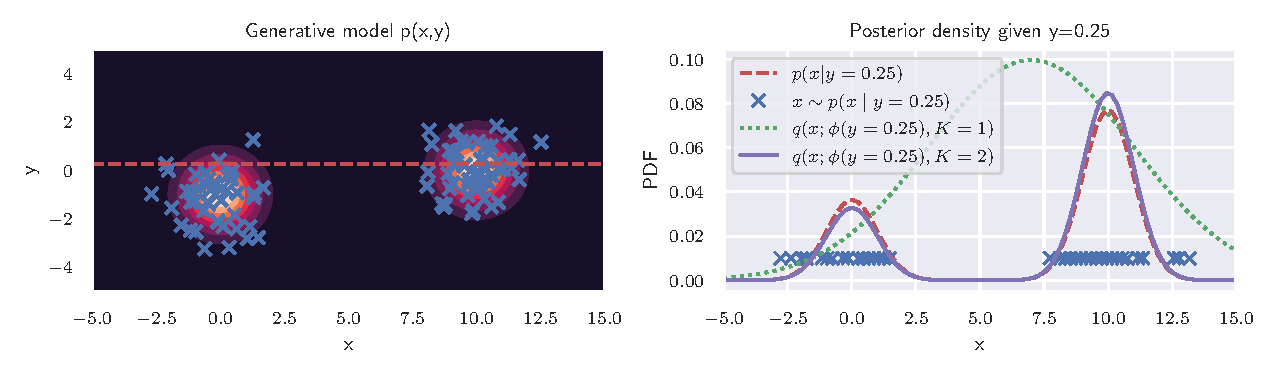
\includegraphics[width=\textwidth,trim=0 20 305 0,clip]{../Figures/intuition.pdf}
          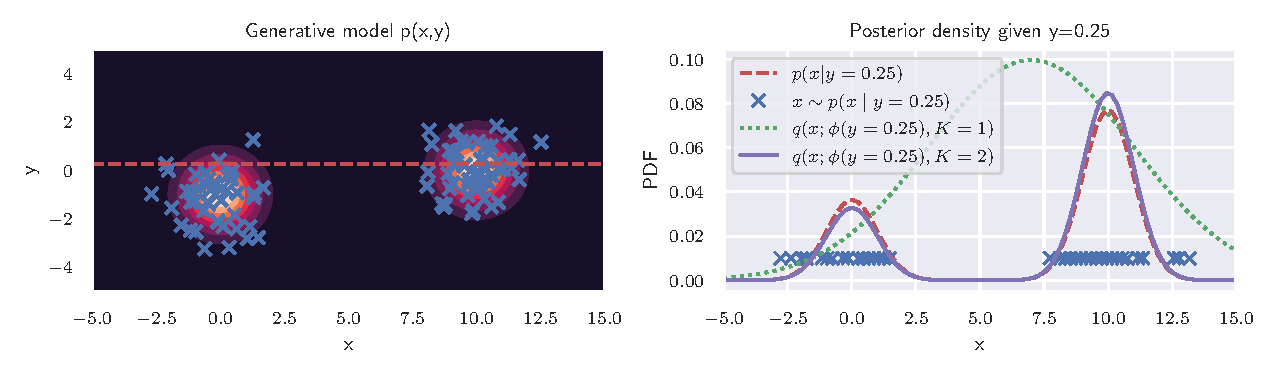
\includegraphics[width=\textwidth,trim=305 10 0 10,clip]{../Figures/intuition.pdf}
          \caption{
            Generative samples $(x,y) \sim p(x,y)$ yield information about the posterior
            $p(x \mid y)$ for multiple values of $y$, enabling amortized inference
          }
        \end{figure}
      \end{block}

      %----------------------------------------------------------------------------------------

      \hrule~\\
      \begin{singlespace}
        \rmfamily{\footnotesize{
            Presented at the 24\textsuperscript{th}\,International Conference
            on Artificial Intelligence and Statistics (AISTATS) 2021, San
            Diego\@. Copyright 2021\/ by the author(s).
          }}
      \end{singlespace}

    \end{column} % End of the first column

    \begin{column}{\sepwid}\end{column} % Empty spacer column

    \begin{column}{\twocolwid} % Begin a column which is two columns wide (column 2)


      %----------------------------------------------------------------------------------------
      %	IMPORTANT RESULT
      %----------------------------------------------------------------------------------------

      % \begin{alertblock}{High Level Model}

      %   Analysis tools:
      %     Semantic interpretation of specificity of LSTM hidden states via plotting gate activations for inputs
      %     What would Bach do? MAP estimate of next note
      %     Fixing LSTM weights and optimizing the inputs

      %   Training, unrolling, BPTT
      %   Sampling

      %   Implementation: keras, tensorflow

      % \end{alertblock}

      %----------------------------------------------------------------------------------------


      %----------------------------------------------------------------------------------------
      %	One-pass polyphonic
      %----------------------------------------------------------------------------------------

      % \begin{block}{Learning a conjugate posterior}
      %   \begin{itemize}
      %     \item Given initial seed, generate entire chorale
      %     \item Baseline: n/a, subjective evaluation
      %     \item Experiments:
      %           \begin{itemize}
      %             \item Bi-axial and grid architectures
      %             \item Convolutional vs recurrent dimensions
      %           \end{itemize}
      %   \end{itemize}

      %   \begin{figure}
      %     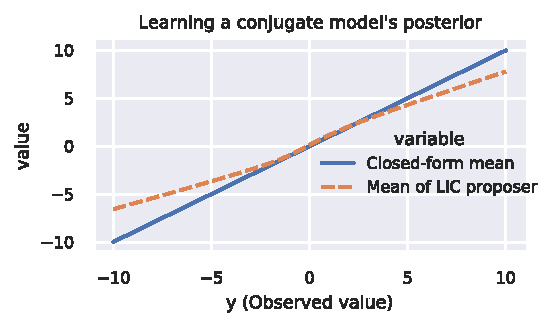
\includegraphics[width=0.95\linewidth]{../Figures/normal_normal_mean_type1.pdf}
      %     \caption{}
      %   \end{figure}
      % \end{block}

      % \begin{block}{Bi-modal GMM}
      %   \begin{itemize}
      %     \item MAP : what would Bach do?
      %     \item Interpreting hidden state activations
      %     \item Enhance ``Bach-ness'' of input
      %   \end{itemize}

      %   \begin{figure}
      %     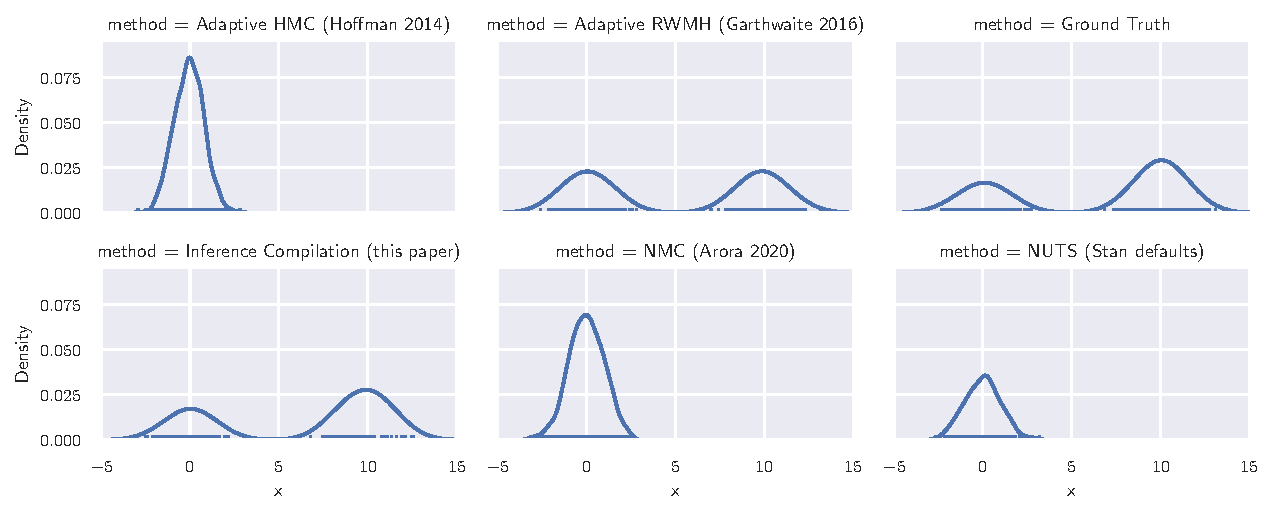
\includegraphics[width=0.95\linewidth]{../Figures/mode_escape.pdf}
      %     \caption{}
      %   \end{figure}
      % \end{block}

      %----------------------------------------------------------------------------------------

      \begin{block}{LIC's architecture and training}
        \begin{itemize}
          \item Run probabilistic program forwards to generate $n$ joint samples $(x,y) \sim p(x,y)$
          \item Minimize Monte-Carlo estimate of inclusive KL-divergence
                \[
                  \mathbb{E}_{y \sim p(y)} KL(p(x \mid y), q(x))
                  \approx \frac{1}{n} \sum_{i=1}^n \log \frac{p(x_i \mid y_i)}{q(x_i;\phi)}
                  \propto \frac{1}{n} \sum_{i=1}^n \log \frac{p(x_i, y_i)}{q(x_i;\phi)}
                \]
        \end{itemize}
        \begin{figure}
          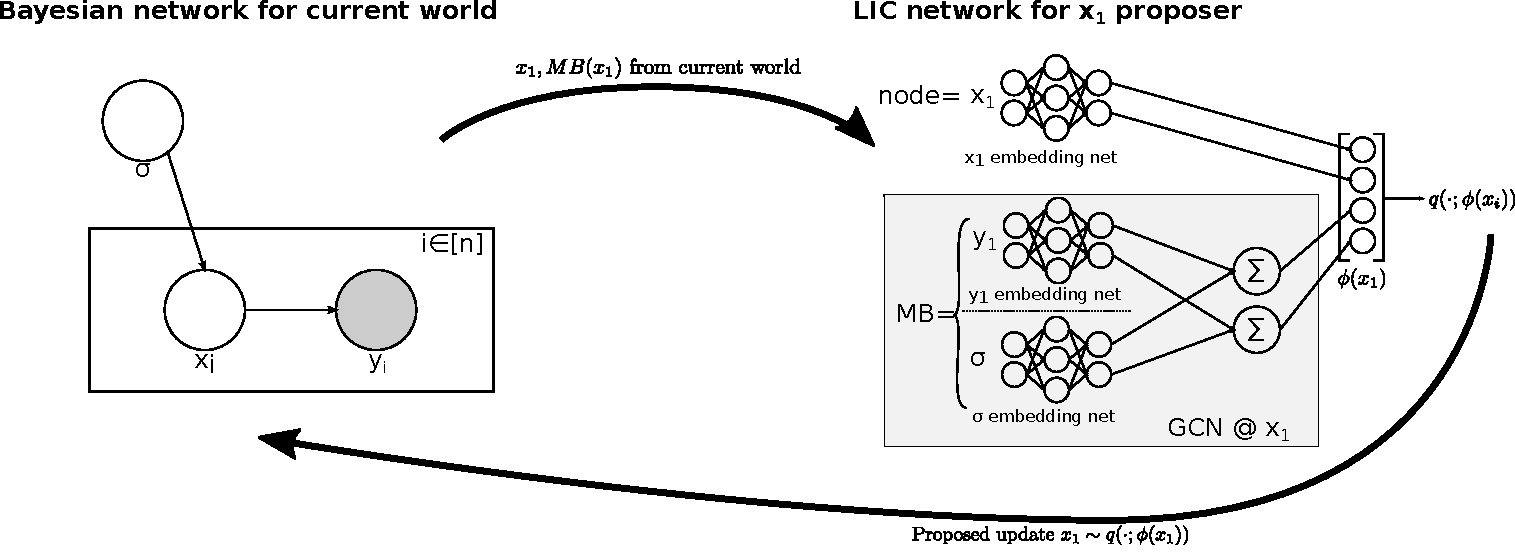
\includegraphics[width=0.75\linewidth]{../Figures/lic_overview.pdf}
          \caption{LIC's architecture for a proposal distribution over
            latent $x_i$ conditioned on $y_i$ and with parent $\sigma$}
        \end{figure}
      \end{block}
      \vspace{-2cm}

      \begin{block}{Bayesian logistic regression and $n$-schools}
        \begin{columns}[t]
          \begin{column}{0.5\textwidth}
            Bayesian logistic regression (BLR)
            \newline
            \begin{align*}
              \vec{\beta} & \sim \cN_{d+1}(\vec{0}_{d+1}, \diag(10, 2.5\vec{1}_{d}))            \\
              y_i         & \mid \vx_i \simiid \text{Bernoulli}(\sigma(\vec{\beta}^\top \vx_i)) \\
              \sigma(t)   & = (1 + e^{-t})^{-1}
            \end{align*}
          \end{column}
          \begin{column}{0.5\textwidth}
            $n$-schools, a generalization of $8$-schools \cite{rubin1981estimation}
            used for Bayesian meta-analysis at a large internet company
            \begin{align*}
              \beta_0     & \sim \text{StudentT}(3, 0, 10)                                                                         \\
              \tau_{i}    & \sim \text{HalfCauchy}(\sigma_i) \qquad \text{for}~i \in [\text{district}, \text{state}, \text{type}]  \\
              \beta_{i,j} & \sim \cN(0, \tau_i)  \qquad \text{for}~i \in [\text{district}, \text{state}, \text{type}], j \in [n_i] \\
              y_k         & \sim \cN(\beta_0 + \sum_i \beta_{i,j_k}, \sigma_k)
            \end{align*}
          \end{column}
        \end{columns}

        \begin{figure}
          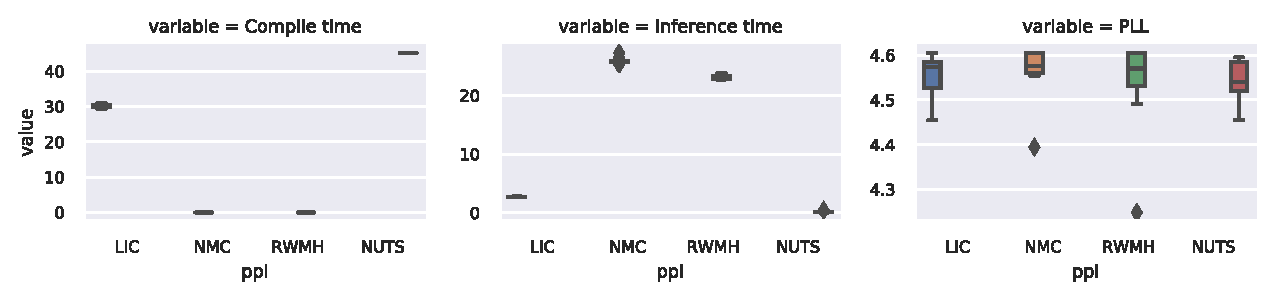
\includegraphics[width=0.475\linewidth,trim=17 0 205 0,clip]{../Figures/blr_pll_type1.pdf}
          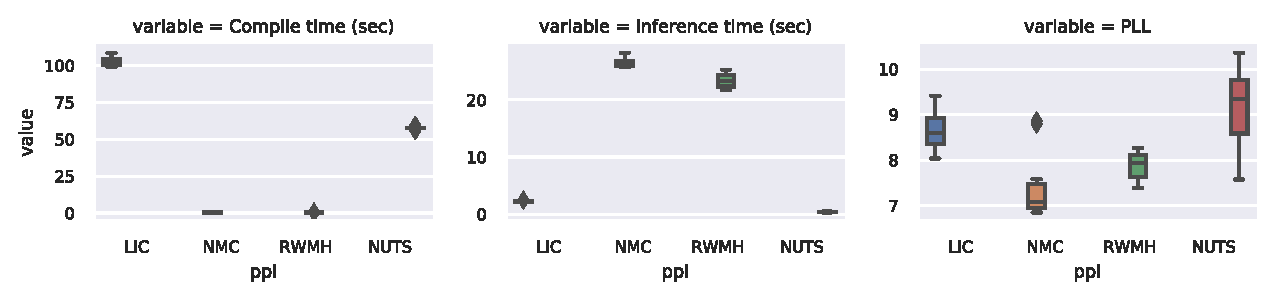
\includegraphics[width=0.485\linewidth,trim=17 0 205 0,clip]{../Figures/nschools_pll_type1.pdf}
          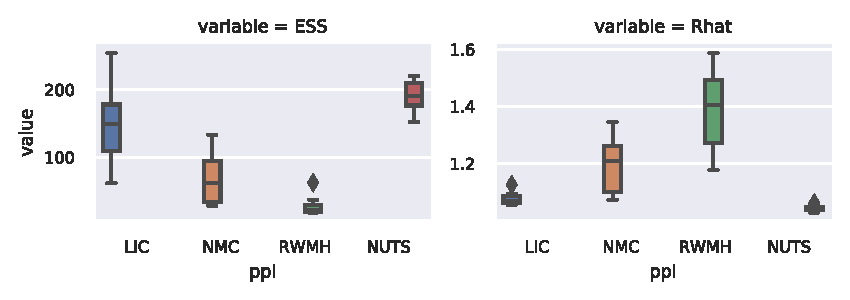
\includegraphics[width=0.475\linewidth,trim=17 0 0 0,clip]{../Figures/blr_ess_rhat_type1.pdf}
          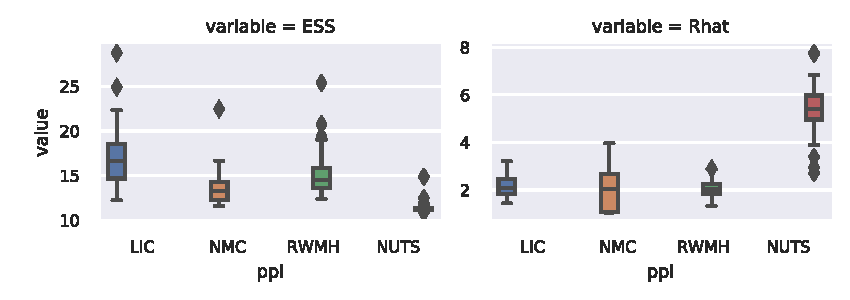
\includegraphics[width=0.485\linewidth,trim=27 0 0 0,clip]{../Figures/nschools_ess_rhat_type1.pdf}
          \caption{Empirical results for Bayesian logistic regression (left) and $n$-schools (right),
            compile time (seconds, lower is better, only applicable to LIC and NUTS), inference time (seconds, lower is better), effective sample size
            (higher is better), and $\hat{R}$ \cite{brooks1998general} (lower is better)}
        \end{figure}
      \end{block}

      %----------------------------------------------------------------------------------------


    \end{column} % End of the second column

    \begin{column}{\sepwid}\end{column} % Empty spacer column

    \begin{column}{\onecolwid} % The third column

      %----------------------------------------------------------------------------------------
      %	Status
      %----------------------------------------------------------------------------------------

      \begin{block}{Robustness to nuisance parameters}
        A version of Program 1 from \cite{harvey2019attention} illustrates
        LIC's improved robustness to nuisance parameters compared
        to \cite{pyprob2020}:
        \begin{lstlisting}[language=Python]
x = sample(Normal(0, 10))
for _ in range(100):
  nuisance = sample(Normal(0, 10))
y = sample(Normal(0, 10))
observe(obs**2, 
  likelihood=Normal( x**2 + y**2, 0.1))
        \end{lstlisting}
        \vspace{1cm}
        \begin{figure}
          \centering
          \begin{tabular}{lccc}
            \toprule
                   & \# params & compile time & ESS   \\
            \midrule
            LIC    & 3,358     & 44 sec.      & 49.75 \\
            PyProb & 21,952    & 472 sec.     & 10.99 \\
            \bottomrule
          \end{tabular}
        \end{figure}
      \end{block}

      %----------------------------------------------------------------------------------------
      %	REFERENCES
      %----------------------------------------------------------------------------------------

      \begin{block}{References}

        \nocite{*} % Insert publications even if they are not cited in the poster
        \footnotesize{
          \bibliographystyle{unsrt}
          \bibliography{./refs.bib}
        }

      \end{block}

      %----------------------------------------------------------------------------------------
      %	ACKNOWLEDGEMENTS
      %----------------------------------------------------------------------------------------

      \setbeamercolor{block title}{fg=red,bg=white} % Change the block title color

      \begin{block}{Acknowledgements}

        \small{\rmfamily{Feynman Liang is supported by a NPSC Graduate Fellowship.
            This work was done during an internship at Facebook.}} \\

      \end{block}

      %----------------------------------------------------------------------------------------
      %	CONTACT INFORMATION
      %----------------------------------------------------------------------------------------

      \setbeamercolor{block alerted title}{fg=black,bg=norange} % Change the alert block title colors
      \setbeamercolor{block alerted body}{fg=black,bg=white} % Change the alert block body colors

      \begin{alertblock}{Contact Information}

        \begin{itemize}
          \item \href{https://github.com/feynmanliang/lightweight-inference-compilation}{github.com/feynmanliang/lightweight-inference-compilation}
          \item \href{mailto:feynman@berkeley.edu}{feynman@berkeley.edu}
        \end{itemize}

      \end{alertblock}

      % \begin{center}
      %   
\includegraphics[width=0.5\linewidth]{Figures/UCBwordmark.png}
      % \end{center}

      %----------------------------------------------------------------------------------------

    \end{column} % End of the third column

  \end{columns} % End of all the columns in the poster

\end{frame} % End of the enclosing frame

\end{document}
